\documentclass[11pt,a4paper]{article}
\usepackage{amsmath}
\usepackage{amsthm}
\usepackage{amssymb}
\usepackage[margin=2cm]{geometry}
%\usepackage{thmbox}
\usepackage{graphicx}
\usepackage[dvipsnames,usenames]{color}
\usepackage{url}
\usepackage{comment}
\usepackage{amsmath, amsthm, amssymb,enumerate}

%\usepackage{enumerate}
%\usepackage{titlesec}
%\usepackage{Rvector}
%\usepackage{mathabx}
\newcommand{\qrq}{\quad\Rightarrow\quad}
\newcommand{\qarq}{\quad&\Rightarrow\quad}
\newcommand{\alp}{\alpha}
\newcommand{\claim}{{\underline{\it Claim:}}~~}
\newcommand{\dbR}{\mathbb{R}}
\newcommand{\ndimr}{\mathbb{R}^n}
\newcommand{\vare}{\varepsilon}
\newcommand{\since}{\because\;}
\newcommand{\hence}{\therefore\;}
\newcommand{\en}{\par\noindent}
\newcommand{\fn}{\footnotesize}

\newcommand{\sect}[2]{#1~~{\mdseries\tiny(#2)}}

\renewcommand{\(}{\left(}
\renewcommand{\)}{\right)}

\let \ds=\displaystyle

\usepackage{xeCJK}
\setCJKmainfont[AutoFakeBold=5,AutoFakeSlant=.4]{標楷體}

%\usepackage{fancyhdr}
%\pagestyle{fancy}
%\renewcommand{\headrulewidth}{0pt}

\renewcommand{\thesection}{Lecture \arabic{section}}
\renewcommand{\thesubsection}{\Roman{subsection}}

\usepackage[T1]{fontenc}

%%%% F U N C T I O N %%%%%
\newcommand{\abs}[1]{\left|#1\right|}
\newcommand{\norm}[1]{\left\|#1\right\|}
\newcommand{\inn}[1]{\left<#1\right>}
\newcommand{\f}[1]{f\!\left(#1\right)}
\newcommand{\g}[1]{g\!\left(#1\right)}
\newcommand{\h}[1]{h\!\left(#1\right)}
\newcommand{\x}[1]{x\!\left(#1\right)}
\newcommand{\D}[1]{D\!\left(#1\right)}
\newcommand{\N}[1]{N\!\left(#1\right)}
\renewcommand{\P}[1]{P\!\left(#1\right)}
\newcommand{\R}[1]{R\!\left(#1\right)}
\newcommand{\V}[1]{V\!\left(#1\right)}
\newcommand{\function}[2]{#1\!\left(#2\right)}
\newcommand{\functions}[2]{\left(#1\right)\!\left(#2\right)}

\definecolor{light-gray}{gray}{0.95}
\newcommand{\textfil}[1]{\colorbox{light-gray}{\large\color{Red} #1}}


\renewcommand{\title}{Numerical Optimization with applications\\
	CHAPTER 17: Penalty and Augmented Lagrangian Methods}
\renewcommand{\author}{104021601 林俊傑\\104021602 吳彥儒\\104021615 黃翊軒}
\renewcommand{\maketitle}{\begin{center}\textbf{\Large\title}\\[6pt] {\author}\\[6pt] {\color{Gray}\footnotesize January 15, 2017}\end{center}}
\newcommand{\blue}[1]{{\color{blue}#1}}


\renewcommand{\labelenumi}{(\alph{enumi})}

\newcommand{\Exercise}[2]{\textbf{Exercise #1.} \textit{#2}}
\newtheorem{exercise}{Exercise}

%\parskip=11pt

\begin{document}

  \maketitle

\section*{17.1 THE QUADRATIC PENALTY METHOD}
Given the original constrained optimization problem
\begin{align}
\min_xf(x) \quad \text{subject to } c_i(x) = 0 ,\quad i \in \mathcal{E}, \quad c_i(x)\ge 0, \quad i \in \mathcal{I},
\end{align}
we could define the corresponding quadratic penalty function as
\begin{align}
	Q(x;\mu) := f(x)+\frac{\mu}{2}\sum_{i \in \mathcal{E}}c^2_i(x)+\frac{\mu}{2}\sum_{i\in \mathcal{I}}\left( \left[c_i(x) \right]^- \right)^2, 
\end{align}
where $\mu>0$ and $[y]^-$ is the abbreviated symbol of $\max(-y,0)$.

If we take a sequence $\mu_k \nearrow \infty$ into the quadratic penalty function, we could find that $Q(x;\mu_k)$ deverges if $x$ is infeasible. The larger $\mu_k$ is, the severer constraint violations we panalize. As a result, the minimizer of the quadratic penalty function $Q(x;\mu_k)$ is closer to the feasible region as $k$ increases.
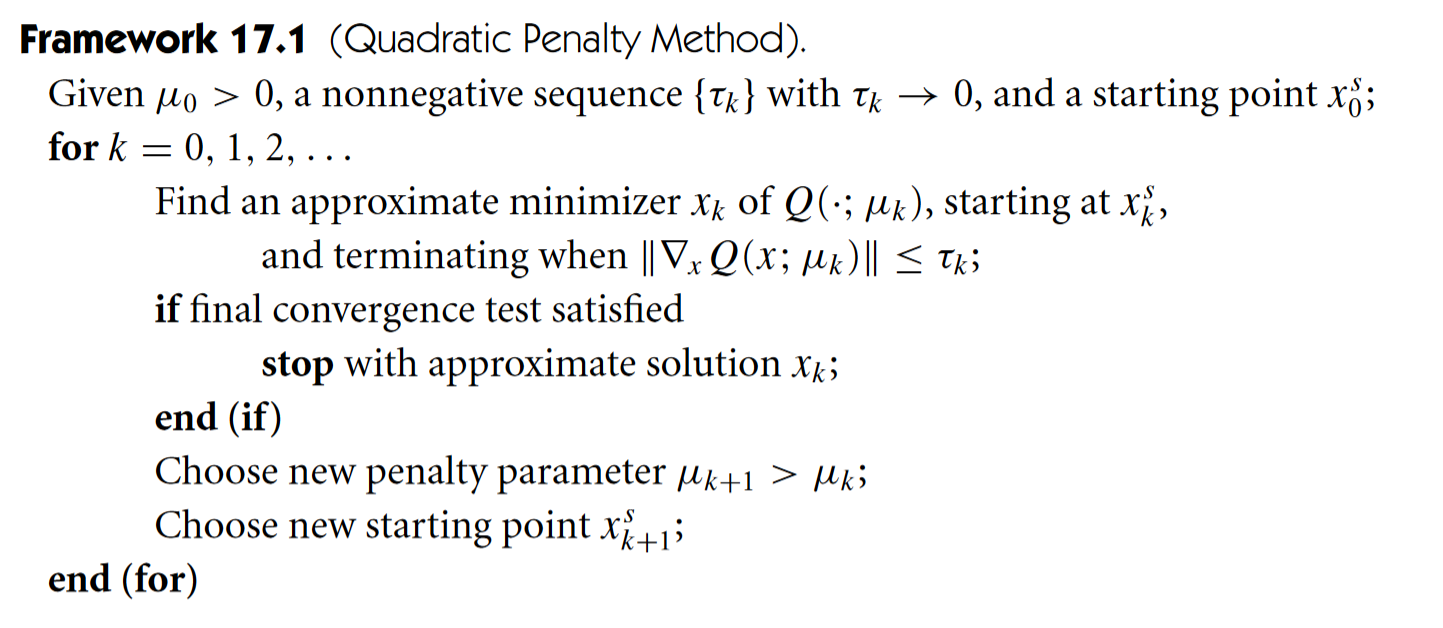
\includegraphics[scale=0.6]{fram17_1}

We have two theorems to support the convergence of Framework 17.1.

\textbf{Theorm 17.1} states that the global minimizer $x_k$ of quadratic penalty function $Q(x;\mu_k)$ converges to the constrained optimization problem $x$, i.e. $x_k\rightarrow x$.

\textbf{Theorm 17.2} states that if $\tau_k \rightarrow 0$ and $x_k$ only satisfies $$\|\nabla_xQ(x;\mu_k)\|\le \tau_k,$$ then $$x_k\rightarrow x^*,$$ where $x^*$ is a stationary point of $\|c(x)\|^2$. Besides, if $\nabla c_i(x^*)$ is linearly independent, then $$\lim_{k\rightarrow \infty}-\mu_kc_i(x_k) = \lambda^*_i \quad \forall i \in \mathcal{E}$$ and $(X^*,\lambda^*)$ satisfy the KKT conditions.

\subsection*{Practical problems}
Even if $\nabla^2f(x^*)$ is well-conditioned, the Hessian $\nabla^2_{xx}Q(x;\mu_k)$ might become ill-conditioned as $\mu_k \rightarrow \infty$. 

By defining $$A(x)^T = (\nabla c_i(x))_{i \in \mathcal{E}}$$ and considering equality constraints only, we have
$$\nabla^2_{xx}Q(x;\mu_k) = \nabla^2f(x)+\sum_{i \in \mathcal{E}}\mu_kc_i(x)\nabla^2 c_i(x) + \mu_kA(X)^TA(X).
$$
From \textbf{Theorem 17.2}, we have $$\mu_kc_i(x)\approx -\lambda^*_i$$ for $x$ near a minimizer.
Hence, we obtain $$\nabla^2_{xx}Q(x;\mu_k) \approx \nabla^2_{xx}\mathcal{L}(x,\lambda^*) + \mu_kA(X)^TA(X).$$
We find that $\nabla^2_{xx}Q(x;\mu_k)$ have problems with ill-conditioning since the second term diverges as $\mu_k \rightarrow \infty$. 

For Newton's method step
$$
\nabla^2_{xx}Q(x;\mu_k)p = \nabla_{x}Q(x;\mu),
$$ we can apply a reformulation

\[
\begin{pmatrix}
	\nabla^2f(x)+\sum_{i \in \mathcal{E}}\mu_kc_i(x)\nabla^2 c_i(x) & A(x)^T\\
	A(x) & -(1/\mu_k)I
\end{pmatrix}
\begin{pmatrix} p \\ \mu A(x)p \end{pmatrix}
=
\begin{pmatrix} -\nabla_xQ(x;\mu_k)\\ 0 \end{pmatrix}
\]
to avoid the ill-conditioning since $p$ solves both systems. Note that this system has dimension $n+|\mathcal{E}|$ rather than
n.



\section*{17.2 NONSMOOTH PENALTY FUNCTIONS}
A penalty function ia called {\em exact} if, for certains coice of penalty parameters, the minimizer $x^\star$ is the exact solution of the original constrained optimization problem. Nevertheless, the quadratical penalty function is not exact. In this section, we introduce the {\em nonsmooth} penalty functions.\\
A popular nonsmooth penalty function is the $l_1$ {\em penalty function} defined by
\begin{equation}\label{E:22}
\phi_1(x;\mu)=f(x)+\mu\sum_{i \in \mathcal{E}}|c_i(x)|+\mu\sum_{i \in \mathcal{I}}[c_i(x)]^-.
\end{equation}
The next two theorems establish the {\em exactness} of (\ref{E:22}).\\
\textbf{Theorm 17.3} states that if $x^\star$ is a strictly local minimizer of (1), with Lagrange miltipliers $\lambda^\star$. Then $x^\star$ is a local minimizer of (\ref{E:22}) \quad$\forall~\mu > \mu^\star$, where
\begin{equation}\label{E:23} 
\mu^\star= \norm{\lambda^\star}_\infty 
\end{equation}
\textbf{Theorm 17.4} states that if $\hat{x}$ is a stationary points of $\phi_1(x;\mu)$ for all $\mu$ large enouth. Then, $\hat{x}$ is either satisfying KKT conditions for (1) or it is an infeasible stationary points.\\
Define the measure of infeasibility
\begin{equation}\label{E:27}
 h(x)=\\sum_{i \in \mathcal{E}}|c_i(x)|+\\sum_{i \in \mathcal{I}}[c_i(x)]^- 
\end{equation}
Then, we can develope an algorithm framwork via the $l_1$ penalty funtion.\\
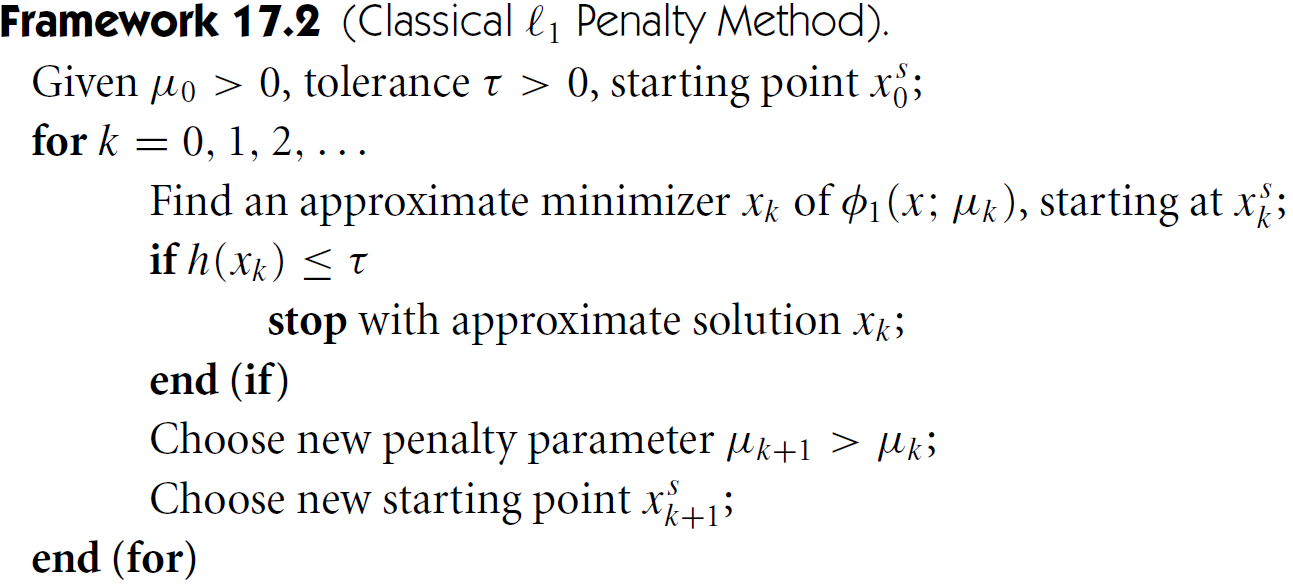
\includegraphics[scale=0.33]{fram17_2}\\
Since $\phi_1(x;\mu)$ is nonsmooth, the minimization will be difficule. However, we can transform $\phi_1(x;\mu)$ into a smooth model.
\subsection*{A PRATICAL $l_1$ PENALTY METHOD}
As we did for the unconstrained optimization problem, we can transform (\ref{E:22}) into a smooth model by replacing $f$ by its Taylor expension and $c_i$ by its linearization,as follows:
\[ q(p;\mu)=f(x)+\bigtriangledown f(x)^Tp+\frac{1}{2}p^TWp+\mu\sum_{i \in \mathcal{E}}|c_i(x)+\bigtriangledown c_i(x)^Tp|+\mu\sum_{i \in \mathcal{I}}[c_i(x)+\bigtriangledown c_i(x)^Tp]^- \]
where $W$ is an approximation of Hessian about $f$ and $c_i$.
The function $q(p;\mu)$ is still not smooth, but we can reformulate it into a smooth quadratic optimization problem by introducing some new variables, as follows:
\begin{equation}\label{E:31}
\begin{split}
\min_{p,r,s,t} \quad & \quad f(x)+\frac{1}{2}p^TWp+\bigtriangledown f(x)^Tp+\mu\sum_{i \in \mathcal{E}}|r_i+s_i|+\mu\sum_{i \in \mathcal{I}}t_i \\
subject~to  \quad &~ \bigtriangledown c_i(x)^Tp+c_i(x)=r_i-s_i, \quad i \in \mathcal{E}\\
&~ \bigtriangledown c_i(x)^Tp+c_i(x) \geq -t_i, \quad i \in \mathcal{I}\\
&~ r,s,t\geq 0
\end{split}
\end{equation}
Even after adding a trust region constraint $\norm{p}_\infty \leq \bigtriangleup$, (\ref{E:31}) is still a quadratic problem. It can be solved by a quadratic programming solver.
\subsection*{A GENERAL CLASS OF NONSMOOTH PENALTY METHODS}
Exact nonsmooth penalty funtions can use other norms.
\begin{equation}\label{E:32}
\phi(x;\mu)=f(x)+\mu \norm{c_\mathcal{E}(x)}+\mu \norm{[c_\mathcal{I}(x)]^-}
\end{equation}
Framework 17.2 can work on these penalty functions by simply redefinind the measure of infeasibility (\ref{E:27}) as $h(x) = \norm{c_\mathcal{E}(x)}+\norm{[c_\mathcal{I}(x)]^-}$.\\
The properties garguaranteed by Theorem 17.3 and Theorem 17.4 can be extended to the general class (\ref{E:32}).In Theorem 17.3, we replace $\mu^\star$ in (\ref{E:23}) by
\[ \mu^\star = \norm{\lambda^\star}_D, \]
where $\norm{•}_D$ is the dual norm of $\norm{•}$. Theorem 17.4 applies without modification.



\section*{17.3 AUGMENTED LAGRANGIAN METHOD: EQUALITY CONSTRAINTS}
In section 17.1, we know that even $\mu_{k}$ is large, the approximate minimizer $x_{k}$ of the quadratic penalty function $Q(x;\mu_{k})$ may be infeasible, the violation of $c_{i}(x)\approx-\lambda_{i}^{*}/\mu_{k}.$ To make the approximate solution $x_{k}$ closer to the feasible region, we introduce the Augmented Lagrangian function:
\begin{align}
\mathcal{L}_{A}(x,\lambda;\mu):=f(x)-\sum_{i\in\mathcal{E}}\lambda_{i}c_{i}(x)+\frac{\mu}{2}\sum_{i\in\mathcal{E}}c_{i}^{2}(x)
\end{align}
Use the fact of Theorem 2.2 and (17.17), and rearranging the expression, we have $c_{i}(x_{k})\approx-\frac{1}{\mu_{k}}(\lambda_{i}^{*}-\lambda_{i}^{k})$, the violent of $x_{k}$ is much smaller than $\frac{1}{\mu_{k}}$.  We can set the Lagrangian multiplier vector of the next step $\lambda_{i}^{k+1}=\lambda_{i}^{k}-\mu_{k}c_{i}(x_{k}),$ for all $ i\in \mathcal{E}$.\\
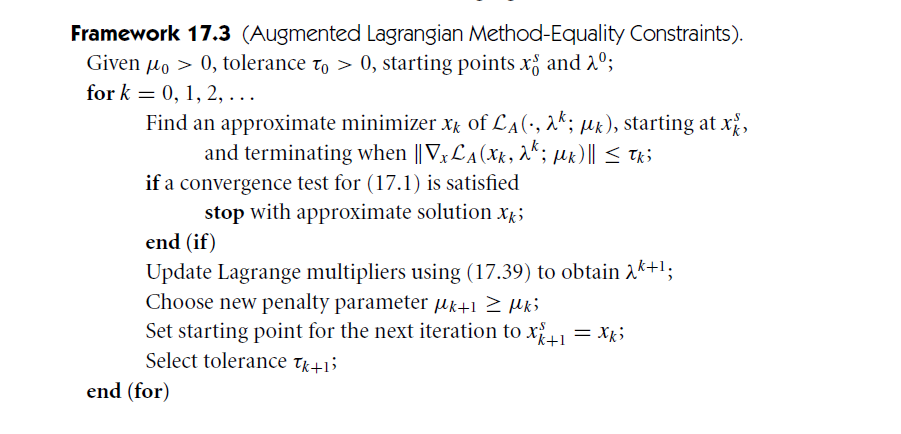
\includegraphics[scale=0.6]{fram17_3}\\
\textbf{Theorm 17.5} states that if we know the exact Lagrangian multiplier $\lambda^{*}$, then the solution of (1) is a strict minimizer of $\mathcal{L}_{A}(x,\lambda;\mu)$ for $\mu$ large enough. Even though we only have a "good" estimate of $\lambda^{*}$, we can still get  a good estimate of $x^{*}$ by minimizing  $\mathcal{L}_{A}(x,\lambda;\mu)$ with large $\mu$.\\
\textbf{Theorm 17.6} states the advantage of the augmented Lagrangian method. Different from the quadratic penalty method, we can get a good approximation of $x^{*}$ if $\lambda_{k}$ is close to $\lambda^{*}$ or if the penalty parameter $\mu_{k}$ is large. On the other hand, by (17.46), we can improve the accuracy of $\lambda^{*}$ by choosing a large $\mu_{k}$.\\
\section*{17.4 PRACTICAL AUGMENTED LAGRANGIAN METHOD}
In section 17.3, we only discuss the problem with equality constrains. Now for the general case, there are three useful formulations.\\
\textbf{Bound-Constrained Formulation}\\
Use the slack variable $s_{i}$ to turn inequalities into equalities. That is
\begin{align*}
c_{i}(x)-s_{i}=0,~~~s_{i}\geq0,~~~ \forall i\in \mathcal{I}
\end{align*}
We can reformulate the problem into
\begin{align*}
\min_{x\in\mathbb{R}^{n}}f(x)~~s.t.~~~~c_{i}(x)=0,~~~i=1,2,...,m,~~~l\leq x\leq u
\end{align*}
The Bounded-constrained Lagrangian will be:
\begin{align*}
\min_{x}\mathcal{L}_{A}(x,\lambda;\mu)=f(x)-\sum_{i=1}^{m}\lambda_{i}c_{i}(x)+\frac{\mu}{2}\sum_{i=1}^{m}c_{i}^{2}(x)~~~s.t.~~~ l\leq x\leq u
\end{align*}
Solve this problem and update $\lambda$ and $\mu$ repeatedly.\\
\textbf{Linearly Constrained Formulation}\\
LCL method is to solve the subproblem of minimizing the augmented Lagrangian function subject to linearization of the constrains.
\begin{align*}
\min_{x}~~~&F_{k}(x)\\
s.t.~~~&c(x_{k})+A_{k}(x-x_{k})=0,~~l\leq x\leq u. 
\end{align*}
where
\begin{align*}
c_{i}^{-k}(x)=c_{i}(x)-c_{i}(x_{k})-\bigtriangledown c_{i}(x_{k})^{T}(x-x_{k}).
\end{align*}
Current Augmented Lagrangian funciton
\begin{align*}
F_{k}(x)=f(x)-\sum_{i=1}^{m}\lambda^{k}_{i}c^{-k}_{i}(x)+\frac{\mu}{2}\sum_{i=1}^{m}[c^{-k}_{i}(x)]^{2}
\end{align*}
\textbf{Unconstrained Formulation}\\
Suppose the problem has no equality constrain, i.e. $\mathcal{E}=\emptyset$, then we can rewrite the problem as
\begin{align*}
\min_{x \text{ feasible}}f(x) = \min_{x\in \mathbb{R}^{n}}F(x)
\end{align*}
where
\begin{align*}
F(x)=\max_{\lambda\geq0}\lbrace f(x)-\sum_{i\in \mathcal{I}}\lambda_{i}c_{i}(x)\rbrace
\end{align*}
Note that if x is feasible, $F(x)=f(x)$ and $\lambda_{i}$ should be zero. Otherwise $F(x)$ turns to infinity, and $\lambda_{i}$ can be chosen arbitrary large. Consequently, $F$ is not smooth, so it is not practical to minimize directly. We replace F by a smooth approximated function
\begin{align*}
\widehat{F}(x;\lambda^{k},\mu_{k})=\max_{\lambda\geq 0}\lbrace f(x)-\sum_{i\in\mathcal{I}}\lambda_{i}c_{i}(x)-\frac{1}{2\mu_{k}}\sum_{i\in\mathcal{I}}(\lambda_{i}-\lambda_{i}^{k})^{2}
\end{align*}
where the last term can enforce the mew maximizer $\lambda$ close to the previous estimate $\lambda^{k}$.\\
By above, we can obtain the explicit maximization of $\lambda$. Then we have 
\begin{align*}
\widehat{F}(x;\lambda^{k},\mu_{k})=f(x)+\sum_{i\in\mathcal{I}}\psi(c_{i}(x),\lambda^{k}_{i};\mu_{k})
\end{align*}
where the function$\psi$ is defined as
\begin{align*}
\psi(t,\sigma;\mu):=
\begin{cases}
-\sigma t+\frac{\mu}{2}t^{2}~&\text{if} t-\sigma/\mu\leq 0,\\
-\frac{1}{2\mu}\sigma^{2} &\text{otherwise,}
\end{cases}
\end{align*}
Hence, we can obtain $x_{k}$ by minimizing $\widehat{F}$, and update Lagrange multiplier estimates repeatedly.





\end{document} 